\section{Theorie}

\begin{flushleft}
    Ein Schwingkreis, welches aus zwei Energiespeichern besteht (Kondensator mit der Kapazität \textbf{C} sowie eine Spule mit der Induktivität \textbf{L}), wird ein Energiebetrag zwischen den beiden Speichern übertragen.
    Anders als bei einem RC-Kreis, kann der Schwingkreis periodische Schwingungen ausführen.
    Dies schließt darauf, dass der Strom \textbf{I}(t) sein Vorzeichen periodisch wechselt.
    Der Kondensator wird aufgeladen und dabei entsteht ein elektrisches Feld zwischen den Kondensatorplatten.
    Beim Entladen fließt der Strom durch die Spule und es entsteht somit ein Magnetfeld.
    Sobald der Strom nachlässt, word der Kondensator mit umgekehrter Polarität wieder aufgeladen.  
    Dies führt dazu, dass der Energieaustausch zeitlich unbegrenzt erhalten bleibt.
\end{flushleft}

\begin{flushleft}
    Wird jedoch ein Widerstand \textbf{R} in das Schaltsystem eingebaut, so nimmt die gesamte elektrische
    Energie mit der Zeit ab. Die Amplitude des Stroms sowie die Spannung am Kondensator nehmen eine
    monoton fallende Funktion ein. Man spricht hier von einer gedämpften Schwingung.
\end{flushleft}

 
\begin{figure}[H]
    \centering
    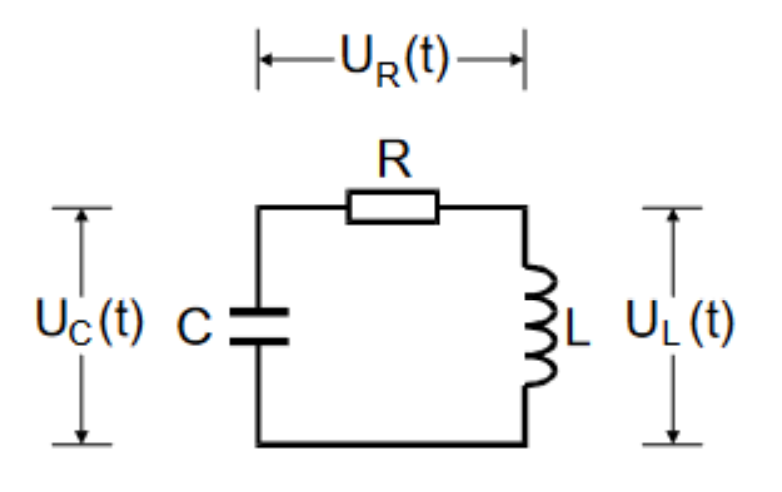
\includegraphics[width=90mm]{bilder/Ab1.png}
    \caption{Die Darstellung eines RCL-Kreises \cite[1]{GedUErzSch}. \label{Abbildung1}}
\end{figure}


\begin{flushleft}
    Wie in der Abbildung \ref{Abbildung1} zu sehen, gelten für die drei Spannungen $\text{U}_{\text{C}}$, $\text{U}_{\text{R}}$ und $\text{U}_{\text{L}}$ nach dem zweiten Kirchhoffschen Gesetz:
\end{flushleft}


\begin{equation}
    \text{U}_\text{R}(\text{t}) + \text{U}_\text{C}(\text{t}) + \text{U}_\text{L}(\text{t})=0\,. \label{1}
\end{equation}


\begin{align}
    \intertext{Die einzelnen Teile können durch den Strom I(t) ausgedrückt werden:}
    \text{U}_{\text{R}}(\text{t}) = \text{RI}(\text{t})\notag \\ 
    \text{U}_{\text{C}}(\text{t}) = \frac{\text{Q}(\text{t})}{\text{C}}\notag \\
    \text{U}_{\text{L}}(\text{t}) = \text{L}\,\frac{\text{dI}}{\text{dt}} = \text{L}\,\dot{\text{I}}\,.\notag \\
    \intertext{Daraus folgt}
    \text{L}\,\dot{\text{I}} + \text{RI} + \frac{\text{Q}}{\text{C}} = 0\,, \quad \text{mit} \quad \text{I} = \frac{\text{dQ}}{\text{dt}}\,.\notag
    \intertext{Durch Umformen ergibt sich für Differentialgleichungen zweiter Ordnung:}
    \ddot{\text{I}}(\text{t}) + \frac{\text{R}}{\text{L}}\,\dot{\text{I}}(\text{t}) + \frac{1}{\text{LC}}\,\text{I}(\text{t}) = 0\,.\notag
    \intertext{Mit der Lösung:}
    \text{I}(\text{t}) = e^{-2\,\pi\,\mu\,\nu\,\text{t}}(\text{A}_{1}e^{-2\,\pi\,\nu\,\text{t}} + \text{A}_{2}e^{-2\,\pi\,\nu\,\text{t}})\,,\notag
    \intertext{mit}
    \mu = \frac{R}{4\pi L} \label{2}
    \intertext{sowie}
    \nu = \frac{1}{2\,\pi}\,\sqrt{\frac{1}{\text{LC}} - \frac{\text{R}^2}{4\,\text{L}^2}}\,. \label{3}
\end{align}

\begin{align}
    \intertext{$\nu$ kann sowohl reel als auch imaginär sein, d.h wir müssen hier zwei Fälle betrachten.
    Für den Fall, dass $\nu$ reel ist, gilt:}
    \frac{1}{\text{LC}} > \frac{\text{R}^2}{4\,\text{L}^2}\,.\notag
    \intertext{Durch Beachtung der Eulerschen Formel kann eine oszillatorische Funktion dargestellt werden:}
    \text{I}(\text{t}) = \text{A}_{0}e^{-2\,\pi\,\mu\,\text{t}} \cos{(2\,\pi\,\nu\,\text{t} + \eta) }\,.\notag
    \intertext{Die folgende Funktion stellt eine gedämpfte Schwingung dar, soll heißen eine harmonische Schwingung, die mit zunehmender Zeit ihre Amplitude exponentiell gegen null verläuft.
    Die Abnahme der Amplitude lässt sich durch die sogenannte Abklingdauer definieren:}
    \text{T}_{\text{ex}}:= \frac{1}{2\,\pi\,\mu} = \frac{2\,\text{L}}{\text{R}}. \label{4}
\end{align}

\begin{align}
    \intertext{Für den Fall, dass $\nu$ imaginär ist, gilt:} 
    \frac{1}{\text{LC}} = \frac{\text{R}^2}{4\,\text{L}^2}\,. \notag
    \intertext{Hierbei liegt ein aperiodischer Grenzfall vor, bei der die Lösung keinen oszillatorischen Anteil mehr besitzt.
    Ein Spezialfall wird in Betracht gezogen, wobei $\nu = 0$ entspricht:}
    \frac{1}{\text{LC}} = \frac{\text{R}_{\text{ap}}^{2}}{4\,\text{L}^2}\,. \label{5}
    \intertext{ Dieser Fall wird aperiodischer Grenzfall genannt, bei dem der Strom I(t) schnell gegen null abfällt.} \notag
\end{align}

\begin{flushleft}
    In einem weiteren Versuch wird eine Wechselspannung zusätzlich an den RLC-Kreis angeschlossen und dabei wird der Einfluss untersucht.
    Nach einer gewissen Einschwingzeit folgt der Oszillator nicht mehr nach seinem Eigenschwingverhalten, sondern in der Erregerfrequenz, hierbei die Frequenz 
    des Wechselstroms mit der Wechselspannung $\text{U}(\text{t}) = \text{U}_{0}\,e^{\text{i} \omega \text{t}}$.
\end{flushleft}

\begin{figure}[H]
    \centering
    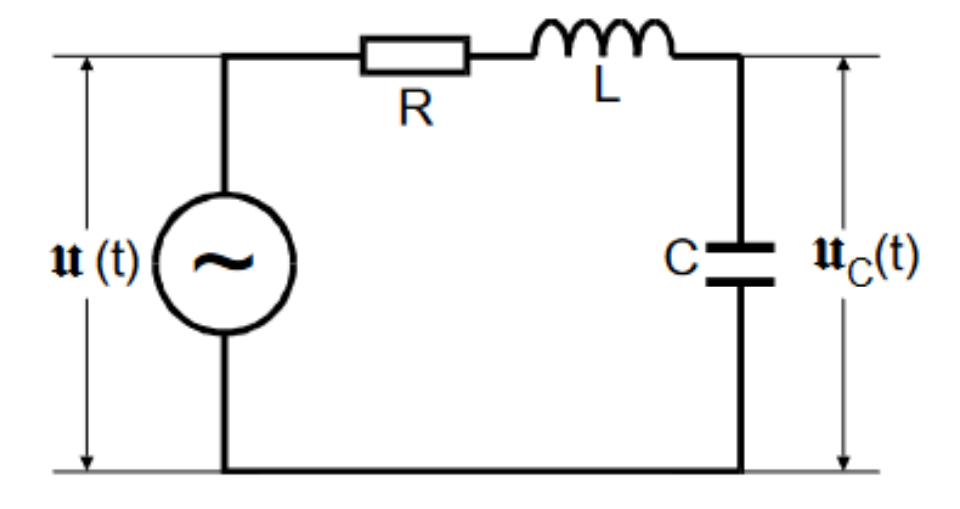
\includegraphics[width=80mm]{bilder/Ab2.png}
    \caption{Die Darstellung einer Erzwungenen Schwingung \cite[6]{GedUErzSch}.\label{Abbildung2}}
\end{figure}


\begin{align}
    \intertext{Die in Gleichung (\ref{1}) aufgestellte Differentialgleichung ändert sich somit zu:}
    \text{LC}\,\ddot{\text{U}}_{\text{C}}(\text{t}) + \text{R}\,\dot{\text{C}}\,\text{U}_{\text{C}}(\text{t}) + \text{U}_{\text{C}}(\text{t}) = \text{U}_{0}\,e^{\text{i} \omega \text{t}}\,. \label{6}
    \intertext{Zudem ergibt sich für die Spannung am Kondensator:}
    \text{U}(\text{t}) = \frac{\text{U}_{0}}{1 - \text{LC}\, \omega^2 + \text{i}\,\omega\,\text{RC}} = \frac{\text{U}_{0}(1 - \text{LC}\, \omega^2 + \text{i}\,\omega\,\text{RC})}{(1 - \text{LC}\, \omega^2)^2 + \omega^2\,\text{R}^2\,\text{C}^2}\,. \notag
    \intertext{Mit der Phasenverschiebung:}
    \tan{(\varphi(\text{t}))} = \frac{\text{Im}(\text{U})}{\text{Re}(\text{U})} = \frac{- \omega\,\text{RC}}{1 - \text{LC}\, \omega^2} \label{7} \\
    \implies \varphi(\text{t}) = \arctan{\left(\frac{-\omega\,\text{RC}}{1 - \text{LC}\, \omega^2}\right)}\,.\label{8}
    \intertext{Die Spannung für den Kondensator kann auch wie folgt aufgeschrieben werden:}
    \text{U}_{\text{C}} (\omega) = \frac{\text{U}_{0}}{\sqrt{(1 - \text{LC}\, \omega^2)^2 + \omega^2 \text{R}^2 \text{C}^2}}. \label{9}
\end{align}


\begin{align}
    \intertext{Dabei wird die Abhängigkeit der Kondensatorspannung von der Erregerfrequenz herausgestellt.
    Wenn $\text{U}_{\text{C}}$ sein Maximum erreicht und somit auch größer als $\text{U}_{0}$ sein kann, dann bezeichnet man dies als Resonanz und die auftretende Frequenz als Resonanzfrequenz $\omega_{\text{res}}$ }
    \omega_{\text{res}} =\sqrt{\frac{1}{\text{LC}} - \frac{\text{R}^2}{2\,\text{L}^2}}\,. \label{10}
    \intertext{Falls sich die Resonanzfrequenz der Kreisfrequenz nähert, dann liegt eine schwache Dämpfung vor mit dem Fall:}
    \frac{\text{R}^2}{2\,\text{L}^2} \ll \frac{1}{\text{LC}}\,. \notag 
    \intertext{Man spricht von einer Resonanzkatastrophe, wenn $\text{R} \to 0$ und $\text{U}_{\text{C,max}} \to \infty $ gehen bei} 
    \text{U}_{\text{C,max}} = \frac{1}{\omega_{0}\,\text{RC}}U_{0} = \frac{1}{\text{R}}\sqrt{\frac{\text{L}}{\text{C}}\,\text{U}_{0}}\,. \label{11}
    \intertext{Dabei wird der Faktor $\frac{1}{\omega_{0}\,\text{RC}}$ als Güte bezeichnet. Die Breite der Resonanzkurve, welche durch die beiden Frequenzen $\omega_{+}$ und $\omega_{-}$ ausgedrückt wird, sinkt bei der Kondensatorspannung $\text{U}_{\text{C}}(\omega)$ um den Faktor $\frac{1}{\sqrt{2}}$.}
    \intertext{Mit} 
    \frac{\text{R}^2}{\text{L}^2} \ll \omega_{0}^2\,, \notag
    \intertext{lässt sich die Breite der Resonanzkurve wie folgt ausrechnen:}
    \omega_{+} - \omega_{-} \approx \frac{\text{R}}{\text{L}}\,. \label{12}
\end{align}

\begin{align}
    \intertext{Für den Fall einer starken Dämpfung gilt:}
    \frac{R^2}{2L^2} \gg \frac{1}{LC}\,. \notag
    \intertext{Betrachtet man die Phasenverschiebung $\varphi(\omega)$, bei denen die Phasenverschiebung die Werte $\frac{\pi}{4}$ 
    oder $\frac{3}{4}\,\varphi$ besitzt, so gilt:}
    \omega_{1,2} =\pm \frac{\text{R}}{\text{L}} \sqrt{ \frac{\text{R}^2}{4\,\text{L}^2} + \frac{1}{\text{LC}}}\,. \label{13}
    \intertext{Daraus folgt}
    \omega_{1} - \omega_{2} = \frac{\text{R}}{\text{L}}. \label{14}
\end{align}